\RequirePackage{mmap}
\documentclass[12pt]{article}
\usepackage[utf8]{inputenc}
\usepackage{geometry}
\geometry{
  margin=1in,
}
\usepackage{amsmath,amsthm,amssymb, listings, color, bm}
\usepackage{mathtools}
\usepackage{changepage}% http://ctan.org/pkg/changepage
\usepackage{enumitem}
\usepackage{csquotes}
\usepackage{fancyhdr}
\usepackage[T1]{fontenc}
\usepackage{titlesec}
\usepackage[absolute]{textpos}
\usepackage[hidelinks]{hyperref}
\usepackage{fontspec}
\usepackage[linesnumbered,ruled]{algorithm2e}
\setmainfont{Latin Modern Roman}
%% \usepackage{setspace}
%% \doublespacing

\renewcommand{\P}{\mathbb{P}}
\newcommand{\E}{\bm{E}}
\newcommand{\Var}{\bm{Var}}
\newcommand{\ul}[1]{\underline{#1}}

\newtheorem{theorem}{Theorem}[section]
\newtheorem{corollary}{Corollary}[theorem]
\newtheorem{lemma}[theorem]{Lemma}
\theoremstyle{definition}
\newtheorem{definition}{Definition}[section]

\DeclareMathOperator*{\argmax}{arg\,max}
\DeclareMathOperator*{\argmin}{arg\,min}

\setlength{\parindent}{0.25in}

\newif\ifextra
\extrafalse

\title{}

\pagenumbering{arabic}

\begin{document}
\pagestyle{fancy}
\fancyhf{} % sets both header and footer to nothin
\cfoot{\thepage}
\renewcommand{\headrulewidth}{1pt}
\lhead{\fontsize{10}{12} \selectfont CSE 446: Machine Learning (Prof. Sham Kakade)\\\textbf{\emph{Section 4: Margin of Separation, SVD}} }
\rhead{\fontsize{10}{12} \selectfont Kaiyu Zheng (TA)\\ \today}

\section{Margin of Separation}
\begin{figure}[h]
  \centering
  \includegraphics[scale=0.8]{figs/margin}
  \caption{Decision boundary and margin. Left: possible decision boundaries. Center: One possible decision boundary with margin $\gamma$. Right: decision boundary that best separates the data $\mathcal{D}$ (with largest margin $\gamma_{\mathcal{D}}$).}
  \label{fig:perceptron}
\end{figure}



\section{Singular Value Decomposition}
\begin{theorem}
  For any given real matrix $A\in\mathbb{R}^{n\times m}$, there exists a unique set of matrices $U, S, V$ such that
  \begin{equation}
    A = USV^T
  \end{equation}
  where $U\in\mathbb{R}^{n\times n}$ and $S\in\mathbb{R}^{n\times p}$ and $V\in\mathbb{R}^{p\times p}$ $U^TU=I$ and $V^TV=I$. This is called the \emph{singular value decomposition} of $A$.
\end{theorem}
$U$ and $V$ are orthonormal matrices. $S$ is a diagonal matrix\footnote{More precisely, it is a rectangular diagonal matrix because $n$ may not equal to $p$. Still, $S_{ij}=0$ if $i\neq j$.}. The elements in $S$ are called \emph{singular values} of $A$. The eigenvectors of $A^TA$ are columns of $V$, and the eigenvectors of $AA^T$ are columns of $U$. The entries in $S$ are positive, and sorted in decreasing order ($S_{11}\geq S_{22}\geq\cdots$).

% The $n$-dimensional column vectors of $U$ are called \emph{left-singular vectors}, and the $p$-dimensional column vectors of $V$ are called \emph{right-singular vectors}. Singular value decomposition can be viewed as a series of transformations to 

\subsection{Connection to Principal Component Analysis}

The goal of principal component analysis (PCA) is to represent observations $X\in\mathbb{R}^{n\times d}$ using vectors called \textbf{principal components} and arrive at $Z\in\mathbb{R}^{n\times k}$ such that $k<d$ and best preserves variance of $X$.
This is useful because typically we are presented with data of extremely high dimensions (millions), and not all features are useful. We hope to reduce the dimensionality of feature space, so that (1) there are fewer parameters to learn, (2) we can better understand which (uncorrelated) features are useful to represent the data, and (3) we can potentially visualize the data.

\bibliography{references}
\bibliographystyle{plain}

\end{document}

